\documentclass[sigconf]{acmart}

\usepackage{hyperref}

%\usepackage{endfloat}
%\renewcommand{\efloatseparator}{\mbox{}} % no new page between figures

\usepackage{booktabs} % For formal tables

\settopmatter{printacmref=false} % Removes citation information below abstract
\renewcommand\footnotetextcopyrightpermission[1]{} % removes footnote with conference information in first column
\pagestyle{plain} % removes running headers


\begin{document}
\title{Hadoop and MongoDB in support of Big Data Applications and Analytics}


\author{Sushant Athaley}
\affiliation{%
  \institution{Indiana University}
}
\email{sathaley@iu.edu}

% The default list of authors is too long for headers}
\renewcommand{\shortauthors}{G. v. Laszewski}


\begin{abstract}
Big data processing is beyond the capability of traditional tools. It requires specialized tools to handle the volume, velocity, and variety of big data. We explore Haddop and MongoDB technically as a tool and how they provide support/help in big data analytics.

\end{abstract}

\keywords{i523, hid302, big data, Hadoop, MongoDB, HDFS, MapReduce}

\maketitle

\section{Introduction}
The emergence of big data challenges also gave rise to the various technologies which can be used to solve big data problem. Typically to solve big data, we need to consider two types of technologies, data capture and storage, and data analysis. We evaluate capabilities of two popular technologies Hadoop and MongoDB to understand their features and power to solve big data problem. We get started with the section \emph{Big Data} which captures big data definition and characteristics. Section \emph{Hadoop} provides an introduction to the technology and subsections \emph{Hadoop Common, HDFS, YARN, MapReduce} explores technology in detail. Section \emph{Big Data Support} captures how Hadoop supports big data analytics along with the real-life examples. We then explore MongoDB through section \emph{MongoDB} which further drill down to the technology using sections \emph{Architecture, Data Model, Data Management, Data Visualization, and Security}. Section \emph{Big Data Support} captures how MongoDB supports big data analytics along with the real-life examples. Section \emph{Power of Two} captures how both technologies can be used together to solve big problems. Section \emph{Conclusion} concludes the study. 

\section{Big Data}
Big Data is defined in lot many different ways but one of the interesting ways it has been defined is in terms of three V's which are Volume, Velocity, and Variety. Big data is generated in great \emph{volume} typically in the gigabyte or more which makes data processing difficult. Data \emph{velocity} has been increased due to the real-time data streaming from various applications like social media or different type of sensors recording data continuously. Big data comes in \emph{variety} of format like structured or unstructured data. Data varies in various format like text, pictures, audio, videos, 3D, social media and so on. These big data characteristics pose challenges in terms of overall data lifecycle management. Some of the examples of big data usage are the recommendation service, predictive analytics, data analytics, pattern identification, and machine learning. Traditional systems are good for small or medium data processing but unable to provide support for the big data. Big data need specialized technologies and tools to handle its characteristics. The technologies which can solve big data problem should have capabilities like distributed computing system, massively parallel processing, NoSQL, and analytical database \cite[Ch.\ 1, p. 4]{AchariShiva2015HE}. Can Hadoop or MongoDB be those technologies who can provide that support?  

\section{Hadoop}
Apache foundation describes Hadoop as ``The Apache Hadoop software library is a framework that allows for the distributed processing of large data sets across clusters of computers using simple programming models. It is designed to scale up from single servers to thousands of machines, each offering local computation and storage. Rather than rely on hardware to deliver high-availability, the library itself is designed to detect and handle failures at the application layer, so delivering a highly-available service on top of a cluster of computers, each of which may be prone to failures'' \cite{www-hadoop}. In other words, Hadoop provides a framework to store data in the distributed manner and provides the capability to run data analysis in the distributed way.

``Currently Hadoop project includes following modules:
\begin{itemize}
\item {\bf Hadoop Common}: The common utilities that support the other Hadoop modules.
\item {\bf Hadoop Distributed File System (HDFS)}: A distributed file system that provides high-throughput access to application data.
\item {\bf Hadoop YARN}: A framework for job scheduling and cluster resource management.
\item {\bf Hadoop MapReduce}: A YARN-based system for parallel processing of large data sets'' \cite{www-hadoop}.
\end{itemize}

\subsection{Hadoop Common}
Hadoop Common is the collection of the utilities to support the Hadoop modules. This is the core package which provides essential and basic service of the framework.

\subsection{Hadoop Distributed File System (HDFS)}
Hadoop Distributed File System (HDFS) is the default distributed file system provided by the Hadoop. HDFS serves as storage mechanism in the Hadoop framework. HDFC specifically designed to process large data set and run on low-cost hardware. It is highly fault-tolerant which contains the mechanism for quick fault detection and auto recovery. HDFS is designed to port across heterogeneous hardware and software platform. It does data computation on the same node instead of moving data to the server which is faster as well as avoid network congestion. It provides scalability by adding or removing nodes in the HDFS cluster and can support hundreds of nodes in single cluster \cite{www-hdfs-arch}. Figure \ref{f:hdfs-arch} shows HDFS architecture.
\begin{figure}[!ht]
  \centering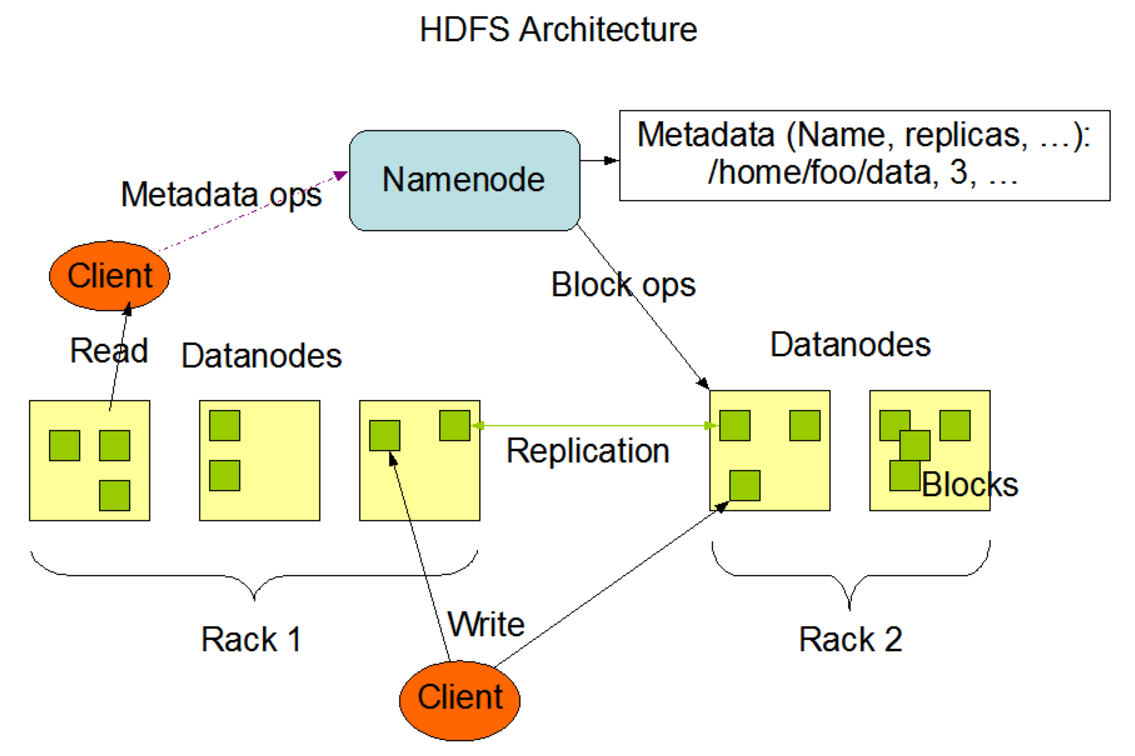
\includegraphics[width=\columnwidth]{images/hdfsArch.PNG}
  \caption{HDFS Architecture \cite{www-hdfs-arch}}\label{f:hdfs-arch}
\end{figure}

HDFS is based on master/slave architecture where NameNode is the master server and DataNodes are the slave nodes. There can be only one NameNode server which manages file system namespace and all read-write requests. NameNode doesn't store any data but contains all the meta-data about files and DataNodes. DataNode contains actual data and they can be multiple in numbers usually one per node. DataNodes are responsible for the create, delete, replicate of the data blocks on the node as per the instruction by the NameNode. DataNode also sends block-report to NameNode which has a list of all blocks on the DataNode. DataNode sends the heartbeat message to NameNode which helps in identifying the failure nodes. If the heartbeat is not received by NameNode in specified interval then that DataNode is marked as dead and NameNode usage different DataNode. Figure \ref{f:hdfs-read} and \ref{f:hdfs-write} depicts read and write in HDFS respectively.

\begin{figure}[!ht]
  \centering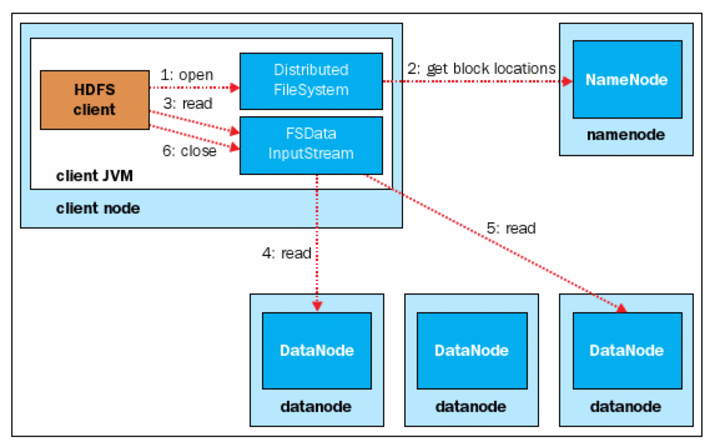
\includegraphics[width=\columnwidth]{images/hdfsRead.PNG}
  \caption{HDFS Read \cite[Ch.\ 3, p. 38]{AchariShiva2015HE}}\label{f:hdfs-read}
\end{figure}

\begin{figure}[!ht]
  \centering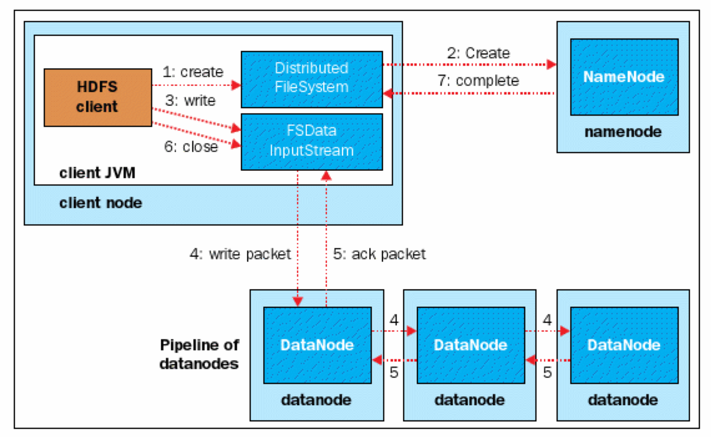
\includegraphics[width=\columnwidth]{images/hdfsWrite.PNG}
  \caption{HDFS Write \cite[Ch.\ 3, p. 39]{AchariShiva2015HE}}\label{f:hdfs-write}
\end{figure}


\subsection{Hadoop YARN}
Hadoop YARN (Yet Another Resource Negotiator) provides cluster resource management which helps in running multiple distributed application in Hadoop. YARN consists of 3 components \emph{ResourceManager (RM), NodeManager (NM)} and \emph{ApplicationMaster (AM)}. ResourceManager is the master process which manages resources across the nodes. NodeManager is responsible for the container and provides resource usage to the ResourceManager. ApplicationMaster is responsible for getting resources from ResourceManager and work with NodeManager to execute the task \cite{www-apache-yarn}. YARN makes it possible to run different applications on Hadoop platform which makes it scalable and integrable \cite[Ch.\ 3, p. 65]{AchariShiva2015HE}.
Figure \ref{f:yarn-arch} shows YARN architecture.
\begin{figure}[!ht]
  \centering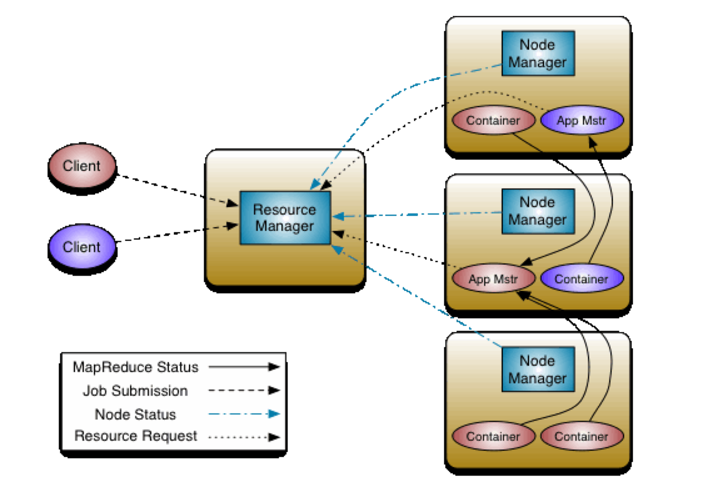
\includegraphics[width=\columnwidth]{images/yarnArch.PNG}
  \caption{YARN Architecture \cite{www-apache-yarn}}\label{f:yarn-arch}
\end{figure}

\subsection{Hadoop MapReduce}
Hadoop MapReduce is a framework which provides the capability to process the vast amount of data in a distributed manner. Processing is done in parallel on various nodes utilizing local machine processor and memory which results in high computation power. The framework provides fault tolerance along with supporting large clusters usually thousands of nodes. Typical framework processing is to split input data into independent chunks and then processed by \emph{map} tasks in parallel. Sort the output of the map task and then provide that as input to \emph{reduce} task for aggregate processing. Two important classes in this framework under package org.apache.hadoop.mapreduce are Mapper and Reducer. They respectively provide map and reduce method to process the data. 

Figure \ref{f:mapreduceex} shows MapReduce process using wordcount example. Each line in the input file is passed to individual mapper class. Mapper class parses the line and sets count for the word. Sort and shuffle consolidate the data and sends it to the reducer. Reducer performs the final word count and provides the output.  
\begin{figure}[!ht]
  \centering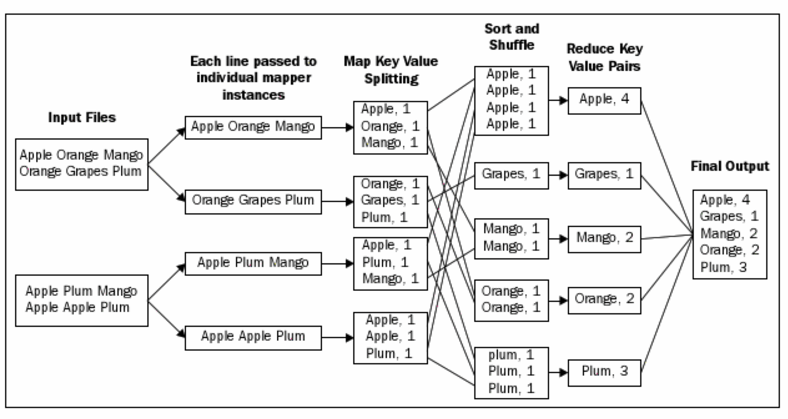
\includegraphics[width=\columnwidth]{images/mapReduceEx.PNG}
  \caption{MapReduce Example \cite[Ch.\ 3, p. 48]{AchariShiva2015HE}}\label{f:mapreduceex}
\end{figure}

\subsection{Big Data Support}
Big data problem solution requires tools which can process the huge amount of data with high computation power. Hadoop provides this capability by processing data in the distributed environment in big clusters using MapReduce and also provides distributed storage system as HDFS. HDFS can be configured in a cluster of hundreds of nodes and can typically store the file in size of gigabytes or terabytes \cite{www-hdfs-arch}. Using CPU and memory of local nodes delivers great computation power. Hadoop also provides high tolerance to the faults and scalability by adding nodes and integration with various technologies. Being open source and configurable on commodity hardware, Hadoop is cost effective and can be used by small industries as well for their big data solution. Hadoop's capability to process large-scale data in parallel within distributed environment makes it one of the best tool for Big Data processing. Hadoop is supported by various sub-projects which together forms Hadoop Ecosystem. Different applications can be integrated with Hadoop depending on the big data problem need to be solved.  
Figure \ref{f:hadoopeco} illustrates Hadoop ecosystem by various layers.
\begin{figure}[!ht]
  \centering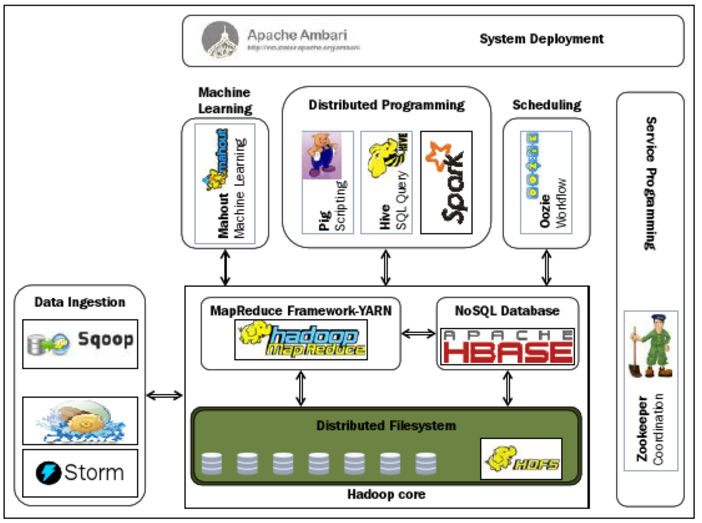
\includegraphics[width=\columnwidth]{images/hadoopEcosys.PNG}
  \caption{Hadoop Ecosystem \cite[Ch.\ 2, p. 26]{AchariShiva2015HE}}\label{f:hadoopeco}
\end{figure}

Yahoo has one of the biggest Hadoop clusters. It has more than 100,000 CPUs in 40,000 computers running Hadoop. Their biggest cluster is of 4500 nodes. Yahoo is using Hadoop in research of Ad systems and web search and also used to do scaling tests to support the development of Apache Hadoop on larger clusters \cite{www-apache-poweredby}.

Facebook uses Apache Hadoop to store copies of internal log and dimension data sources and use it as a source for reporting/analytics and machine learning. They have 2 major Hadoop cluster, a 1100-machine cluster with 8800 cores and about 12 PB raw storage and a 300-machine cluster with 2400 cores and about 3 PB raw storage. Each node has 8 cores and 12 TB of storage \cite{www-apache-poweredby}.

Ebay has 532 nodes Hadoop cluster. They are heavy user of Mapreduce, Apache Pig, Apachae Hive and Apache Hbase. They are using Hadoop for search optimization and research \cite{www-apache-poweredby}. 

\section{MongoDB}
The rise of Big Data started posing challenges on how data can be stored and processed. The inability of the traditional relational database to scale to big data volume and variety gave rose to the NoSQL databases. Based on the concept of one size doesn't fit all, NoSQL implementation comes in 4 different flavors, namely Column/Column Family, document, key-value and graph. MongoDB is one of the popular implementation of the document type NoSQL \cite{Harrison2015}.

\subsection{Architecture}
MongoDB architecture blends best of relational and NoSQL technologies. It is enriched from relational database learning and incorporated new NoSQL features.
Figure \ref{f:mongo-arch} shows MongoDB architectural consideration.
\begin{figure}[!ht]
  \centering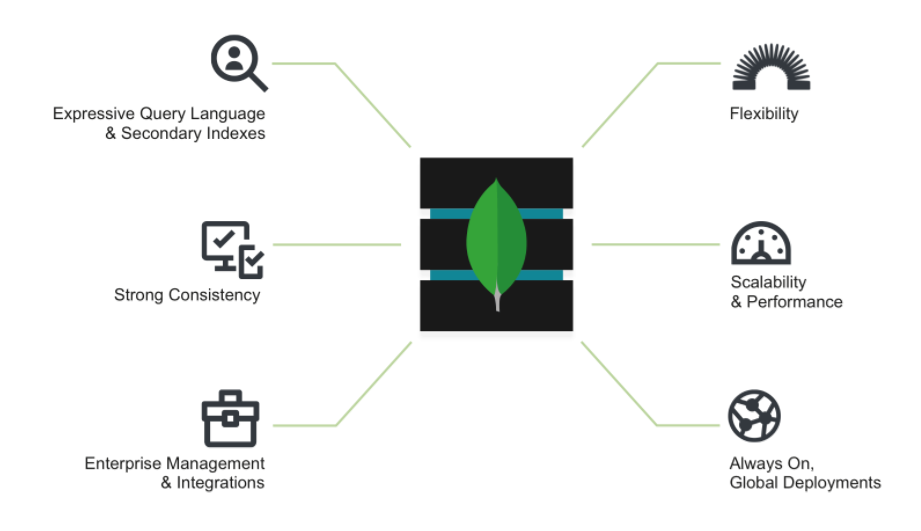
\includegraphics[width=\columnwidth]{images/mongoArch.PNG}
  \caption{MongoDB Architecture \cite{www-mongo-arch}}\label{f:mongo-arch}
\end{figure}
MongoDB provides powerful query language, indexing capability, strong read-write consistency, the capability to integrate with other technologies which they borrowed from the relational database. It also implemented NoSQL features like flexible data model (schema-less),  scalability by sharding or partitioning, and provides high availability by running across the nodes and replication mechanism. MongoDB also provides a multi-model architecture which supports four different storage engines and flexibility to mix and match those storage engines to store data in single MongoDB deployment \cite{www-mongo-arch}.

\subsection{Data Model}
MongoDB stores data as BSON (Binary JSON) document object which is an extension of JSON and includes additional data type such as int, long, date, floating
point, and decimal128. Documents are stored in the collection which is similar to row and table in relational database. The document can vary in structure and usually contains entire object details in the same document. This provides desired structure flexibility in terms of storing data which is not present in the relational database. The document can miss some fields and can be added to the document at any given point time without impacting other documents. Unlike other NoSQL databases, MongoDB provides data validation at the database level. Checks can be enforced at the database level to validate document structure, data types, data ranges and mandatory values \cite{www-mongo-arch}.

\subsection{Data Management}
MongoDB has the capability of horizontal scaling which is referred as Auto-Sharding. In case of data increase, MongoDB distributes data across multiple physical partitions called shards automatically without impacting the application. 

MongoDB is ACID compliant at the document level, the entire document is updated in one transaction or error is thrown.

MongoDB maintains multiple copies of data replica using native replication method. In case of failure, primary replica takes over giving high availability. This is done without impacting the application and is fully automated. 

Ops Manager gives developers, administrators and operations teams monitoring capabilities into the MongoDB service. Featuring charts, custom dashboards, and automated alerting, Ops Manager tracks 100+ key database and systems health metrics including operations counters, memory and CPU utilization, replication status, open connections, queues and any node status.

Disaster recovery is provided using backup and restore mechanism. Backups are taken just a few seconds behind the operational system \cite{www-mongo-arch}.

\subsection{Data Visualization}
MongoDB provides visualization capabilities in MongoDB Enterprise Advanced version using MongoDB Connector for BI. The tool provides the capability to analyze unstructured MongoDB data along with structured SQL database data \cite{www-mongo-arch}.

\subsection{Security}
Security is a growing concern and MongoDB addresses it by providing extensive security features in MongoDB Enterprise Advanced. \emph{Authentication} provides integration with external security mechanism like LDAP, Windows Active Directory, Kerberos etc. \emph{Authorization} can be provided using the user-defined role to access the data also certain data can be masked by using a view. \emph{Audit} capability provides tracking of any command executed on the database. \emph{Encryption} can be used to encrypt the data on the disk, on the network or in backup \cite{www-mongo-arch}. 

\subsection{Big Data Support}
MongoDB is a perfect fit for solving big data problem in terms of database storage. It is capable of handling big data volume and velocity using sharding which scales horizontally. It handles big data variety by providing schema-less data storage. Structured or unstructured, any type of data can be stored in MongoDB. It provides cost benefit as it can be installed on low-cost hardware as well as by cutting down on the development time of the application. It provides ``Analytics and data visualization, text search, graph processing, geospatial, in-memory performance and global replication allow to deliver a wide variety of real-time applications on one technology, reliably and securely'' \cite{www-mongo-arch}.

The City of Chicago uses MongoDB to create smarter and safer city. In just four months, data from Chicago's 15 most crucial department is integrated into MongoDB which provides real-time data analysis to make better decisions. Dashboard created gives querying capability on various department data simultaneously along with twitter data for sentiment analysis \cite{www-mongo-chicago}. 

MongoDB helped online retailer OTTO to improve catalog update time. OTTO now can update catalog within 15 minutes which was earlier could take 12 hours. It helps OTTO to provide a personalized experience to their customer \cite{www-mongo-otto}.

Expedia built scratchpad app using MongoDB to personalize and help their customer by providing previous searches. It saves users all previous travel searches so that users can refer those before finalizing the travel. MongoDB's flexible data structure and ease of development was the selling point for Expedia to use it as database store \cite{www-mongo-expedia}.

\section{Power of Two}
Big data solution requires two types of technology to solve the problem, operational where real-time data is captured and stored, and analytical where this data is used for complex analysis. Frequently both of the technologies are deployed together to solve big data problem. MongoDB and Hadoop are the great choices for operational and analytical technology respectively. MongoDB can be used to store structured/unstructured data and then Hadoop MapReduce can be used to process this data for the analytics. Together they provide the complete and cost-effective solution to the big data problems \cite{www-mongo-bigdata}.

\section{Conclusion}
Hadoop and MongoDB are the front-runner technologies to solve big data problems. The features provided by both technologies are extremely suitable to solve big data problem which requires handling of huge data and great computing power. Distributed nature of both technologies helps data to break across multiple nodes and distributed processing helps process data in parallel. Cost-effective implementation enables to accept these technologies industry-wide. There are a lot of other technologies emerging in the market but Hadoop and MongoDB will be favorite for some time to come.

\begin{acks}

  The authors would like to thank Dr. Gregor von Laszewski for his
  support and suggestions to write this paper.

\end{acks}

\bibliographystyle{ACM-Reference-Format}
\bibliography{report} 

\appendix

\section{Issues}

\DONE{Example of done item: Once you fix an item, change TODO to DONE}

\subsection{Citation Issues and Plagiarism}

    \TODO{Put a space between the citation mark and the previous word}

\subsection{Details about the Figures and Tables}

    \TODO{In case you copied a figure from another paper, you must include a reference to the original in the caption}
    \TODO{Figures should be reasonably sized and often you just need to
  add columnwidth} e.g. \begin{verbatim}/includegraphics[width=\columnwidth]{images/myimage.pdf}\end{verbatim}

re


\end{document}
